
The purpose of this chapter is to give an overview of the research areas
involved in this dissertation. First we explain the fundamental ideas of logic
programming and Prolog; next, tabling by call variance is described, focusing on
the execution strategy and data structures; finally, tabling by call subsumption
and related strategies like \textit{time stamped tries} are explained.

\section{Logic Programming}

Logic programming presents a declarative style of programming based on mathematical
logic and the predicate calculus. It is a very high level programming
paradigm that allows the programmer to focus on the problem at hand, leaving the
steps on \textit{how} to solve the problem to the computer.

In its purest form, logic programming is solely based on Horn Clause Logic \cite{Lloyd-87},
a subset of First Order Logic. Programming in logic can be viewed as
a two step process: (1) first, the theory is formulated as logic clauses,
next (2) we use this theory to search for alternative ways in which an arbitrary query is satisfied.

Logic programming is often mentioned to include the following advantages \cite{Carlsson-PhD}:

\begin{itemize}
  \item \textbf{Simple declarative semantics}: a logic program is simply a collection of predicate logic clauses.
  \item \textbf{Simple procedural semantics}: a logic program can be read as a collection of recursive procedures. In Prolog, for instance, clauses are tried in the order they are written and goals within a clause are executed from left to right.
  \item \textbf{High expressive power}: Logic programs can be seen as executable specifications that despite their simple procedural semantics allow for designing complex and efficient algorithms.
  \item \textbf{Inherent non-determinism}. Since in general several clauses can match a goal, problems involving search are easily programmed in these kind of languages.
\end{itemize}

\subsection{Logic Programs}

A logic program is composed by a set of Horn clauses. Each clause is a disjunction of literals
and contains at most one positive literal. Horn clauses are usually written as

\begin{center}
  $L_{1}, ..., L_{n} \Longrightarrow L  (\equiv \neg L_{1} \vee ... \neg L_{n} \vee \neg L)$
\end{center}

or

\begin{center}
  $L_{1}, ..., L_{n}  (\equiv \neg L_{1} \vee ... \neg L_{n})$
\end{center}

where $n >= 0$ and $L$ is the only positive literal. 

A Horn clause that has exactly one positive literal is called definitive clause; in the Prolog language
it is usually called a \textit{rule}.
A Horn clause without a positive literal is called a \textit{goal}.

Using Prolog's notation, one can write \textit{rules} in the form

\begin{center}
  $L :- L_{1}, ..., L{n}.$
\end{center}

Usually, $A$ is called the \textit{head} of the \textit{rule} and $L_{1}, ..., L_{n}$
the \textit{body} of the \textit{rule}, where each $L_{i}$ is called a subgoal.
A logical \textit{fact} is a special \textit{rule} where the \textit{body} is replaced by \textit{true} symbol:

\begin{center}
  $L.$
\end{center}

Goals are \textit{rules} without the \textit{head} component and are also named as \textit{queries}.


Each literal in Horn clause has the form $p(t_{1}, ..., t_{n})$, where $p$ is the \textit{predicate} symbol or \textit{functor}
and each $t_{i}$ are \textit{terms}. A term can be a \textit{constant} (or \textit{atom}), a \textit{variable}
or a \textit{compound} term. Compound terms follow the predicate structure, recursively.
Variables are assumed to be universally quantified and have the following major characteristics:

\begin{itemize}
  \item Variables are logical variables that can instantiated only once.
  \item Variables are untyped until instantiated.
  \item Variables are instantiated via \textit{unification}, a pattern matching operation that finds the most general common instance of two data objects. 
\end{itemize}

A sequence of clauses with the same functor in the head form a \textit{predicate}. The ordering
of these clauses can have some implications depending on the resolution semantics of the underlying language.
Prolog for instance, uses a top-down resolution mechanism known as \textit{SLD} (Selective Linear Definite) resolution \cite{Lloyd-87}.

SLD starts by matching the first subgoal query to the first clause of the respective predicate,
generating a new query using the body of the clause, which is added to the remaining query subgoals.
During this process a finite set of pairs $\theta$ called \textit{substitution} is built.
Each pair has the form $X = t$, where $X$ is a variable and $t$ is a term. No variable in the left-hand side
of a pair appears on the right-hand side and no two pairs have the same variable as left-hand side \cite{Sterling-94}. 
When the clause body is reused as query, all the variables present in the terms are replaced using the
set $\theta$. 

If unification fails, the next clause of the predicate is tried, in a mechanism called \textit{backtracking}.
This recursive computation fails when there are any more clauses left to try. It succeeds when the subgoal query is empty.

The resolution process is fundamentally non-deterministic and can be viewed as a search within a tree. SLD
does not force any specific search strategy for exploring the tree. Prolog for example, uses a depth-first, one
branch at a time search.

\subsection{Prolog and WAM}
  
Prolog is one of the first logic programming languages and arguably the most successful.
The first implementation of Prolog was Marseille Prolog, developed in 1972 by Alain Colmerauer and Robert Kowalski \cite{Kowalski-74}.

The use of Prolog as a practical and efficient language was made viable by David Warren in 1977, when he built a compiler that could
compete with other languages like Lisp \cite{Warren-77}. Then in 1983, David Warren formulated an abstract machine known as WAM
(\textit{Warren Abstract Machine}) \cite{Warren-83} that is still widely used in modern Prolog implementations.

\subsubsection{Prolog}

Prolog follows the semantics of the SLD resolution through a depth first search strategy.
It starts by choosing the top-most clauses of the predicate and the subgoals are solved
within a left-to-right fashion.

For illustration purposes, we defined the factorial predicate (Listing \ref{factorial_prolog}) that can compute the factorial of
any given number. This predicate has arity of 2, where the first argument is an \textit{input} argument and the second argument
an \textit{output} argument.

\begin{lstlisting}[language=prolog,basicstyle=\footnotesize,float,frame=single,caption={Factorial function in Prolog.},label=factorial_prolog]
factorial(0, 1) :- !.
factorial(N, R) :-
  N > 0,
  N1 is N - 1,
  factorial(N1, R1),
  R is R1 * N.
\end{lstlisting}

Factorial is composed of two clauses, one represents the factorial base case (factorial of 0 is 1) and
the other represents the recursive relation. The second clause first checks if the input number
is positive, to discard non-positive numbers, then computes $N - 1$ and recursively
calls factorial to compute the value of $factorial(N-1)$, finally, the variable $R$ is then unified
to $N * factorial(N-1)$. The first clause uses the \textit{cut} operator that tells the Prolog engine to not explore alternative
clauses, i.e., the factorial of 0 is not to be computed with the recursive relation declared on the second clause.

\begin{figure}[ht]
  \centering
    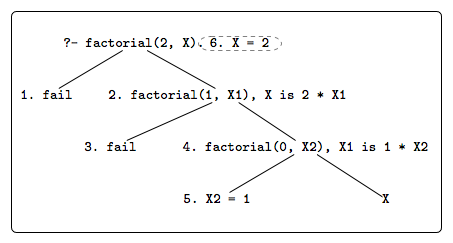
\includegraphics[scale=0.6]{factorial.png}
  \caption{Factorial search tree.}
  \label{fig:factorial_tree}
\end{figure}

Once Prolog finds the first solution (Figure \ref{fig:factorial_tree}), the cut control operator disables further
alternatives, completing the depth first search in the tree.

The cut operator is not the only special instruction in Prolog, more built-in predicates are also available:

\begin{itemize}
  \item \textbf{Meta-logical predicates}: inquire the state of the computation and manipulate terms.
  \item \textbf{Extra-logical predicates}: they can manipulate the Prolog database, adding or removing clauses from
  the program being executed. Input/Output operators are another example of extra-logical predicates.
  \item \textbf{Other predicates}: predicates to perform arithmetic operations, to compare terms, to support debugging, etc.
\end{itemize}

These special operators make programming more practical and useful in real world applications.

\subsubsection{WAM}

The WAM is an abstract machine based on a stack-based architecture with various data areas, registers, and low level instructions
that can be efficiently executed, manipulated and optimized.

The WAM uses the following execution stacks:

\begin{itemize}
  \item \textbf{Code Area}: Contains the compiled instructions.
  \item \textbf{PDL}: A push down list used by the unification process.
  \item \textbf{Trail}: Stores the addresses of the variables that must be reset when backtracking.
  \item \textbf{Stack}: Stores \textit{environment} and \textit{choice point} frames. Environments track the flow control in a program
  and choice points store open alternatives, which are used to restore the state of the computation when backtracking.
  \item \textbf{Heap}: Array of data cells used to store variables and compound terms that cannot
  be stored in the stack.
\end{itemize}

For the registers, WAM defines the following:

\begin{itemize}
  \item \textbf{S}: used during the unification of compound terms.
  \item \textbf{HB}: it is set to contain the value of the register \textbf{H} at the time of latest choice point. This is used to
  determine \textit{conditional} variable bindings that affect variables existing before the creation of the choice point.
  \item \textbf{P}: points to current WAM instruction.
  \item \textbf{CP}: stores the value of \textbf{P} before the current invoked call and it is used to restore the execution point.
  \item \textbf{TR}: points to the top of the trail stack.
  \item \textbf{E}: points to the current active environment.
  \item \textbf{B}: the active choice point.
  \item \textbf{H}: points to the top of the heap stack.
\end{itemize}

WAM instructions can be grouped into four main groups: choice point instructions to manipulate choice points; control
instructions to manage environments and control the execution flow; unification instructions that implement
specialized versions of the unification algorithm; and indexing instructions to efficiently determine which clauses
unify with a given subgoal call.

The WAM being a complex topic has complete books dedicated in explaining its intricacies.
An example is the \textit{Warren's Abstract Machine -- A Tutorial Reconstruction} written by H. A\"{\i}t-Kaci \cite{Aitkaci-91}. 

\section{Tabling}

Despite Prolog's declarativeness and expressiveness, the past few years have seen wide efforts at
solving shortcomings that arise when using SLD resolution.
One proposal that has gained popularity is \textit{tabling} or \textit{tabulation} \cite{Chen-96}.
In comparison to the traditional resolution method, tabling can reduce the search space to cut redundant computations,
avoids looping and has better termination properties \cite{Tamaki-86}.

In a nutshell, tabling is a refinement of the SLD resolution that consists in storing intermediate answers for
subgoals so that they can be reused when a repeated subgoal appears in the resolution process.
The use of tabling enables the programmer to write more expressive, but still valid, logical clauses.

One classical example that is used to demonstrate the need of tabling is presented in Listing \ref{prolog_path}.
This program describes the predicate \textbf{path/2} that can compute reachability between two nodes on a directed graph.
Connections are established as facts using the \textbf{edge/2} predicate.

\begin{lstlisting}[language=prolog,basicstyle=\footnotesize,float,frame=single,caption={\textit{path} program.},label=prolog_path]
:- table path/2.

path(X, Z) :- edge(X, Y), path(Y, Z).
path(X, Z) :- edge(X, Z).

edge(a, b).
edge(b, a).
\end{lstlisting}

\begin{figure}[ht]
  \centering
    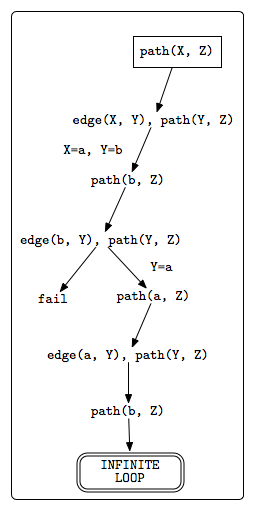
\includegraphics[scale=0.5]{infinite_loop.png}
  \caption{Infinite loop evaluating \textbf{path(X, Z)}.}
  \label{fig:infinite_loop}
\end{figure}

If we tried to evaluate the query goal \textbf{?- path(X, Z).}, traditional Prolog would enter an infinite loop (Figure \ref{fig:infinite_loop})
because the first clause of \textbf{path/2} is right recursive, leading to a repeated call.

\subsubsection{Tabling evaluation}

In this new method of evaluation when a tabled subgoal is first called, a new entry is allocated on the \textit{table space}. Table
entries are used to store subgoal calls but they also store answers found during evaluation. Each time a tabled subgoal is called, we
know if it is a repeated call by inspecting the table space. Nodes in the search space can be classified as:
\textit{generator nodes}, if they are being called for the first time; \textit{consumer nodes} if they are repeated calls;
or \textit{interior nodes} if they are non-tabled subgoals. Generator nodes are matched against the predicate clauses as usual but
consumer nodes are not, instead they consume answers stored in the table space from the respective subgoal.

In Figure \ref{fig:tabling_path} we depict the tabled evaluation of \textbf{?- path(X, Z).}.
Generator nodes are represented by rectangles with double lines and consumer nodes by simple rectangles.
Note that we apply to \textbf{path/2} the \textbf{table} directive to use tabling resolution.

Tabled evaluation starts by inserting a new entry in the table space and by allocating a generator
node to represent \textbf{path(X, Z)} (step 1). Like SLD, \textbf{path(X, Z)} is resolved against the first \textbf{path/2} clause (step 2).
The goal \textbf{edge(X, Y)} is not tabled and is resolved as usual. We use the first \textbf{edge/2} clause with $X = a, Z = b$
and these values are carried to \textbf{path(b, Z)} (step 3). This goal is not yet in the table space, hence we add a new entry for it.

\textbf{path(b, Z)} is then resolved against the first clause of \textbf{path/2} (step 4). \textbf{edge(b, Y)} fails against the first clause but succeeds
with $Y = a$. A new tabled subgoal \textbf{path(a, Z)} is registered in the tabled space (step 6) and resolved against the first clause
of \textbf{path/2} (step 7). This time the \textbf{edge/2} subgoal matches with the first clause ($Y = b$). A repeated tabled subgoal
\textbf{path(b, Z)} is called and the first consumer node is allocated (step 8). As we have no answers for \textbf{path(b, Z)} to consume,
the current evaluation point is \textit{suspended}. Later on, this node can be resumed to consume new answers.

Next, we backtrack to node 7 and try the second \textbf{edge/2} clause, but resolution fails (step 9). We backtrack again, this time to
node 6 to try the second clause of \textbf{path/2} (step 10). Here \textbf{edge(a, Z)} is resolved against the first clause of \textbf{edge/2}
and the solution $Z = b$ is found for the subgoal \textbf{path(a, Z)}. This solution is stored in the table space and forward
execution, propagating the binding $Z = b$ to \textbf{path(b, Z)} (step 12) and the first solution to this subgoal is found and stored.
We continue forward execution and the binding is once again propagated, this time to node 3 (step 13) and we find a solution to
\textbf{path(X, Z)}, $X = a, Z = b$.

\begin{figure}[ht]
  \centering
    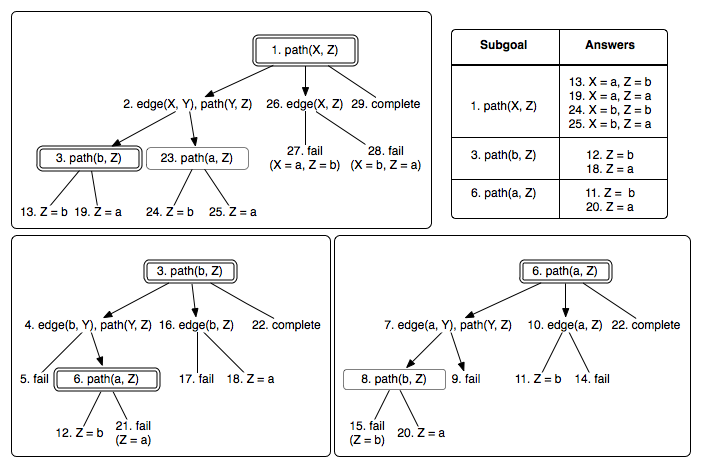
\includegraphics[scale=0.6]{tabling_path.png}
  \caption{Tabled evaluation of \textbf{path(X, Z)}.}
  \label{fig:tabling_path}
\end{figure}

We return to node 10 to try the second clause of \textbf{edge/2}, but we fail (step 14). With no more clauses to try at node 6,
we check wether consumer in node 8 can be resumed. It can, as now it has one unconsumed answer. We resume computation on node 8,
the answer $Z = b$ is consumed and forwarded to subgoal \textbf{path(a, Z)} at node 6. Here, we note that it is a repeated answer
to this subgoal by inspecting the table space, and thus we mark step 15 as \textbf{fail}. Failing repeated answers is crucial
to avoid unnecessary computations and sometimes looping.

At this point, we return again to node 6 but no consumers with unconsumed answers exist and the subgoal cannot be \textit{completed}.
Completing \textbf{path(a, Z)} earlier is not safe, because the consumer under it depends on generator node 3, the subgoal \textbf{path(b, Z)}.
If new answers are found, node 8 should be resumed to consume them, which then can lead to new answers for \textbf{path(a, Z)}.
Completing prematurely would result in lost answers.

We thus backtrack to node 3
to try the second clause (step 16). The first clause of \textbf{edge/2} fails but the second succeeds (step 18), culminating in
a new answer for \textbf{path(b, Z)}, $Z = a$, that is stored. We propagate variable bindings in step 19, generating a new answer
to subgoal \textbf{path(X, Z)}, $X = a, Z = a$.

Every clause in generator node 3 has been tried, so we check if it can be completed. Note that we can safely complete this node,
as it is the youngest generator in which younger consumer nodes have no dependencies on older generator nodes.
Node 3 is called, by definition, a \textit{leader node} and the branch of nodes
below it form a \textit{Strongly Connected Component} (SCC) \cite{Tarjan-72}.

When trying to complete node 3, we verify that node 8 has unconsumed answers. The answer $Z = a$ is fetched (step 20) and propagated
to node 6, generating a new answer to \textbf{path(a, Z)}. This binding is once again propagated, now for node 3 (step 21) but it is
a repeated answer, thus the computation fails. We return back to node 3 to re-attempt completion. This time, no consumers have unconsumed
answers and we can safely complete (step 22). Subgoals \textbf{path(b, Z)} (node 3) and \textbf{path(a, Z)} (node 6) are marked as \textbf{complete}
in the table space and no new answers are accepted.

Next, we backtrack to node 2 to try the second \textbf{edge/2} clause. A new consumer node is allocated (step 23) and answers can be
promptly consumed from the table space. As the subgoal \textbf{path(a, Z)} as been completed before, the consumer node is thus deallocated.
The retrieved answers in step 23 are propagated to node 1 and new answers are generated (step 24 and 25).

We backtrack to node 1 to try the second \textbf{edge/2} clause. Resolution succeeds for both clauses but as the newly found answers
are repeated we fail for both cases (step 27 and 28). The process backtracks again to node 1 and with no more clauses to try,
we attempt completion. As there are no consumer nodes, completion is done (step 29) and computation terminates successfully.

From the described example we can summarize four main operations needed to support tabled evaluation:

\begin{itemize}
  \item The \textit{tabled subgoal call} operation represents a call to a tabled subgoal.
  If the subgoal is already in the tabled subgoal it creates a new consumer node to consume answers.
  If it is a new subgoal call it creates a new generator node and adds a new entry to the table space.
  Each new entry contains an empty set $S$ that will contain answers for the subgoal. 
  
  \item The \textit{new answer} operation adds a new answer $s$ to the table space. If the answer is repeated the operation fails.
  A new answer set $S'$ for the subgoal is generated: $S' \equiv S \cup {s}$.
  
  \item The \textit{answer resolution} operation checks wether new answers from the table space are available for consumption.
  When no new answers are available, the consumer node is \textit{suspended} and execution proceeds using a specific strategy.
  Given the last consumed answer, we determine the unconsumed answer
  set $R$ ($R \subseteq S$) and fetch the element $r \in R$, which is the first element from the set $R$. The last consumed answer
  can be seen as a \textit{continuation} that is stored in each consumer node and is used to determine the next available answer.
  
  \item The \textit{completion} operation determines if a tabled subgoal is \textit{completely evaluated}.
  Only leader nodes can complete themselves and younger generator nodes.
  Once a subgoal is completed the set of answers $S$ is closed and no more answers are accepted; future subgoal calls
  can use the set $S$ without the need to suspend.
\end{itemize}

\subsubsection{Scheduling strategies}

Ensuring efficient execution of tabled evaluation requires different \textit{scheduling strategies}.
During evaluation of the previous example it is very clear that at several points we can choose between
different strategies: continue forward execution, backtrack to interior nodes,
return answers to consumer nodes, or perform completion. Depending on how and when the return of answers is scheduled, different
strategies and searches can be formulated. It is also well known
that using different strategies leads to tremendous effect on performance as some predicates are better suited to specific strategies. 
The most popular scheduling strategies are batched scheduling and local scheduling \cite{Freire-96}.

\textit{Batched scheduling} reduces the need to suspend and move around the search tree by batching the return of answers.
When the engine generates answers, while evaluating a particular goal, the answers are added to the table and the subgoal continues its normal
evaluation until it resolves all available program clauses. Only then the answers are consumed by consumer nodes \cite{Freire-96}.
In some cases, this results in creating dependencies to older subgoals, therefore enlarging the current SCC and delaying completion
to older generator nodes. When backtracking, three situations may arise:

\begin{itemize}
  \item if backtracking to a generator or interior node, try the next available clause.
  \item if backtracking to a consumer node, consume new answers.
  \item if no more clauses are left to try or no more unconsumed answers are available, two options are available:
    \begin{itemize}
      \item if the node is a leader node, attempt completion.
      \item if not, backtrack to a previous branch.
    \end{itemize}
\end{itemize}

For some problems, \textit{local scheduling} is better suited because it tries to evaluate a single exact SCC at a time, preserving the dynamic
SCC ordering during the evaluation. In other words, in a local evaluation, answers are returned to consuming nodes outside of an SCC only after that
SCC is completely evaluated \cite{Freire-96}.
It differs from batched scheduling in that once the answers are found, they are added to the table space, but execution
\textit{fails}. Because this strategy tries to complete sooner rather than later, we can expect less dependencies between subgoals.

\subsubsection{Variant tabling} \label{sec:variant_tabling}

When the subgoal \textbf{path(X, Z)} is called, a check for the presence of this subgoal in the table space is done first.
In the example in Figure \ref{fig:tabling_path}, this was done by checking wether a \textit{variant} of the new goal already
exists in the table. We say that two terms $t_1$ and $t_2$ are variants of each other if they are identical up to renaming of their
variables.

For example, \textbf{path(X, Z)} is variant of the subgoal \textbf{path(X, Y)}, as they represent the same subgoal if we try
to rename their variables to a standardized format. One format was proposed by Bachmair \textit{et al} \cite{Bachmair-93}. Formally,
we have a set $V$ of variables present in a term and a function $renameVar$, such that the first term variable $a \in V$
results in $renameVar(a) = VAR0$ and the following distinct variables are named incrementally ($VAR1, VAR2, ...$).
Using this mechanism, \textbf{path(X, Z)} and \textbf{path(X, Y)} results in \textbf{path(VAR0, VAR1)}. The resulting
standardized subgoal is then checked against the table space to verify if it is a repeated subgoal call.

The variant approach is widely used in tabling systems, but other approaches do exist. One approach named
\textit{call by subsumption} works by checking wether the new goal is subsumed by another goal in the table space.
In other words, we verify if there is a more general subgoal than the one being called. For example
\textbf{path(b, Z)} is subsumed by the subgoal \textbf{path(X, Z)}.

In this approach, instead of creating
a new generator node in step 3, we create a consumer node that would consume answers stored in the subgoal \textbf{path(X, Z)}.
For correct results, it should be clear that the answers used from the table space must unify with \textbf{path(b, Z)}.
Like variant tabling, those new consumer nodes do not expand by using the program clauses, hence the search tree for this new
method will be greatly reduced. This new approach will be throughly explored in Section \ref{sec:subsumption} (Tabling by Call Subsumption).

  \subsection{Yap and XSB}
  
  Yap \cite{system-yap} and XSB \cite{system-xsb} are two well known Prolog systems that implement tabling.
  
  The YAP Prolog System is a high-performance Prolog compiler developed at LIACC, Universidade do Porto.
  It is one of the fastest available Prolog systems and implements a wide range of functionalities: 
  stream I/O, sockets, modules, exceptions, debugging, a C-interface, dynamic code, internal database, DCGs, saved states, co-routining, arrays and threads.
  It is based on the WAM and follows the Edinburgh tradition. Most of the ISO-Prolog standard is implemented.
  
  Tabling in Yap is implemented through the YapTab sub-system \cite{Rocha-03c}, a delaying based tabling engine supporting evaluation of
  definite programs. YapTab follows the seminal SLG-WAM (Linear resolution with Selection function for General logic programs in WAM)
  design from XSB Prolog,
  but it innovates by proposing a new fix-point check algorithm, and by considering that the control of fix-point detection should be
  performed at the level of the data structures corresponding to suspended sub-computations. YapTab was originally designed to achieve
  good results in sequential tabling, but could be extended with the OPTYap engine, for parallel execution \cite{Rocha-05a}.
  Other innovations in YapTab include: support for a dynamic combination of batched and local scheduling and efficient handling of \textit{incomplete
  tables}. Incomplete tables are created when the current computation is pruned from the execution stacks, keeping the pruned subgoals from retrieving
  the complete answer set. Currently, only call by variant checking is supported.
  
  XSB is a research-oriented logic programming system for Unix and Windows based systems. In addition to providing all the functionality
  of the Prolog language, XSB contains several features not usually found in logic programming systems, namely, evaluation according to the
  Well-Founded Semantics (tabling with negation) \cite{Gelder-91} through the use of a delayed-based tabling engine, the SLG-WAM \cite{Chen-96}.
  
  Other features of XSB include: a fully threaded engine, constraint handling for tabled programs on a engine level, a variety of indexing
  techniques, interfaces to other languages, among other things \cite{system-xsb}.
  
  SLG-WAM supports both tabling by variant checking and by subsumption checking. Predicates are available to choose between the two mechanisms.
  XSB also implements a compiler directive, \textbf{auto\_table}, that does static analysis to decide which predicates to table, usually predicates that contain an infinite loop. Tabling by call-subsumption is implemented by a technique called \textit{Time Stamped Tries} \cite{Johnson-99} (described in Section \ref{sec:time_stamped_tries}).
  
  In the next section (Section \ref{sec:table_space}), the table space used to implement
  a call by variance engine is described. Both SLG-WAM and YapTab
  share a lot of similarities in how the table space is organized when using variant checking, hence the description covers
  the common ground between the two systems. Next, in Section \ref{sec:subsumption}, we explore two known mechanisms that
  modify the previous table space for call by subsumption. Those two mechanisms have already been implemented in XSB (\cite{Rao-96} and \cite{Johnson-99}).
  
\subsection{Table Space} \label{sec:table_space}
  
  Implementing a tabling engine on a Prolog system involves the design of compact and time efficient data structures
  to organize the table space. The table space is heavily used throughout the evaluation process in various operations:
  
  \begin{itemize}
    \item to lookup if a subgoal is in the table, and if not insert it;
    \item to verify wether a newly found answer is already in the table, and if not insert it;
    \item to retrieve answers for consumer nodes.
  \end{itemize}
  
  \subsubsection{Tries}
  
  Clearly, the success of tabling is highly dependent on the data structures used.
  Both Yap \cite{Rocha-03c} and XSB \cite{RamakrishnanIV-95} use a trie-based tabling approach.
  
  Tries were initially proposed to index dictionaries \cite{Fredkin-62} and have since been generalized to index recursive data structures
  such as terms. The essential idea underlying a tabling trie is to partition a set $T$ of terms based upon their structure,
  hence common term prefixes are represented only once.
  
  A trie is a tree-structured automaton with the root as the start state and each leaf state is associated with a term in $T$.
  Each state specifies the position to be inspected in the input term on reaching that state.
  The outgoing transitions specify the function symbols expected at that position.
  A transition is taken if the current symbol in the input term matches the symbol of the transition.
  If we recursively reach a leaf state we say that the input term \textit{matches} the term represented by the leaf state.
  A complete path, from the root to a leaf, corresponds to a pre-order traversal of the matching term.
  If no transition can be taken, the lookup operation fails. On the other hand, for an insert operation
  we add a new outgoing transition for the current input symbol and a new node, which is linked to this transition.
  To complete the insert operation, we consume the rest of the input term, until a leaf node is created that represents
  the newly inserted term.
  
  Given the nature of tries, the following conclusions can be made:
  
  \begin{itemize}
    \item it is possible to do a single pass check/insert. If the lookup
    fails, it is possible to complete an insert operation using the last lookup state;
    \item the efficiency and memory consumption of a
    particular trie depends on the percentage of terms that have common prefixes.
  \end{itemize}
  
  When creating transitions for variables, we use the format outlined by Bachmair \textit{et al} \cite{Bachmair-93}.
  It was described in Section \ref{sec:variant_tabling} (Variant tabling).
  
  \begin{figure}[ht]
    \centering
      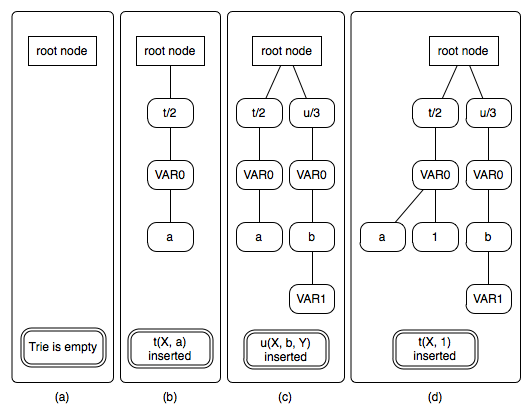
\includegraphics[scale=0.6]{tries.png}
    \caption{Using tries to represent terms.}
    \label{fig:tries_use}
  \end{figure}
  
  The Figure \ref{fig:tries_use} shows a trie with three terms. First, in \textbf{(a)} the trie is represented by a \textit{root node} and has
  no terms. Next, in \textbf{(b)} the term \textbf{t(X, a)} is inserted and three nodes are created that represent each part of the term.
  In \textbf{(c)} a new term, \textbf{u(X, b, Y)} is inserted. This new term differs from the first one and a new distinct branch is created.
  Finally, in \textbf{(d)}, the input term is \textbf{t(Y, 1)} and only a new node needs to be created as this term shares two nodes
  with \textbf{t(X, a)}.
  
  Yap and XSB use two levels of tries to implement tabling:
  
  \begin{itemize}
    \item One level stores subgoal calls for each predicate;
    \item The second level stores answers for a specific subgoal.
  \end{itemize}
  
  \begin{figure}[ht]
     \centering
       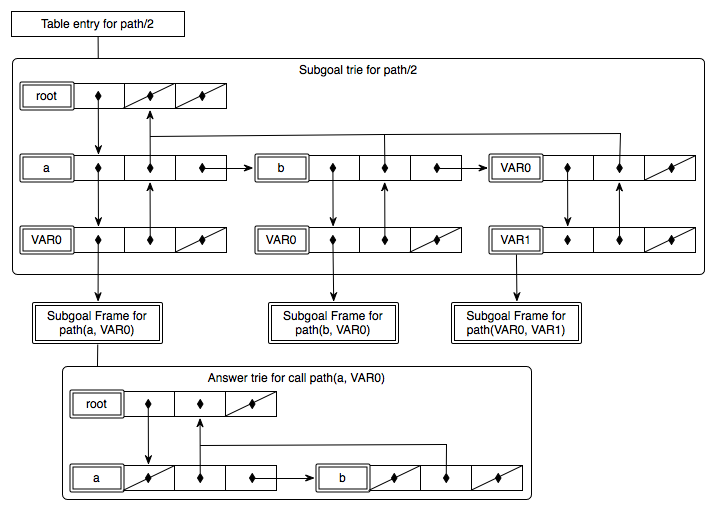
\includegraphics[scale=0.6]{two_level_tries.png}
     \caption{Organizing the table space with tries.}
     \label{fig:table_space_tries}
   \end{figure}
  
  For both levels, each trie node usually contains four fields. The first field represents the \textbf{symbol} (or \textbf{atom})
  of the transition. The second points to the first descendant transition (called the \textbf{child node})
  and the third stores a pointer to the \textbf{parent} node.
  The fourth field points to a \textbf{sibling} node.
  
  When the chain of sibling nodes gets too big, an hashing scheme is dynamically employed to provide direct
  access to nodes, optimizing the search of transitions.
  
  Each tabled predicate contains a \textit{table entry} that points to a \textit{subgoal trie}.
  Only the subgoal arguments are stored.
  Each different call to a tabled predicate corresponds to a unique path through the trie.
  The leaf points to a data structure called \textit{subgoal frame}. The frame stores
  information about the subgoal, namely an entry point to its \textit{answer trie}.
  
  The answer trie stores answers to the subgoal. When inserting answers only substitutions
  for the variables in the call are stored. This optimization is called \textit{substitution factoring} \cite{RamakrishnanIV-95}.
  
  Figure \ref{fig:table_space_tries} shows the table space after evaluating \textbf{path(X, Z)} (example in Figure \ref{fig:tabling_path}).
  Subgoals \textbf{path(X, Z)}, \textbf{path(b, Z)} and \textbf{path(a, Z)} are stored in the \textbf{path/2} subgoal trie.
  Only the answer trie for \textbf{path(a, Z)} is represented. Using substitution factoring only \textbf{Z = b} and \textbf{Z = a}
  were stored.
  
  \subsubsection{Subgoal frames}
  
  A subgoal frame contains general information about the state of a tabled subgoal.
  To access answers, this frames contain a pointer to the root of the answer trie.
  
  A chain of answers used by consumers is also kept in the form of head and tail pointers.
  In XSB, a \textit{answer return list} is built and the consumer has a pointer to the last consumed node of the list.
  In Yap, answers are chained using the \textbf{child} pointer of the leaf answer nodes. Yap's consumers only keep
  the last consumed answer leaf. The last consumed answer pointer is an \textit{answer continuation}. Thus, when
  a consumer needs to verify or consume the next available answer, it uses the continuation to retrieve the next
  answer, following the chain of answers. To load an answer, the trie nodes are traversed in bottom-up order and the answer is reconstructed.
  
  To facilitate memory management, both systems link subgoal frames by storing \textbf{next} and \textbf{previous} pointers in each subgoal frame,
  forming a double linked list.
  
  Information about the current evaluation state of the subgoal is usually kept. Yap has the following states:
  \textit{ready}, \textit{evaluating}, \textit{complete} and \textit{incomplete}.
  
  \subsubsection{Choice Point and Execution}
  
  The YapTab design mostly follows XSB's SLG-WAM approach (\cite{Sagonas-96} and \cite{Sagonas-98}).
  Both introduce the table space,
  a new set of registers, the \textit{freeze registers}, one per stack (local stack, heap and trail);
  an extension of the standard trail,
  called the \textit{forward trail}; and the tabling operations: \textit{tabled subgoal call},
  \textit{new answer}, \textit{answer resolution}, and \textit{completion}.
  
  The set of freeze registers says where stacks are frozen and protect the space belonging to suspended
  computations until the completion of the appropriate SCC takes place. They need to be adjusted
  in two different situations: when a computation suspends, increasing the portion of frozen stacks; and when a completion takes place,
  releasing part of space previously frozen.
  
  The forward trail is used to restore all the variable bindings to their state at the time the computation was suspended.
  Thus, the WAM trail is extended with parent trail entry pointers to create this new trail.
  Also, a new register is created, the \textbf{TR\_FZ} trail freeze register.
  
  The differences between SLG-WAM and YapTab reside in the data structures and algorithms used to control the process of leader detection
  and the scheduling of unconsumed answers. Each engine is described in the next two sections.
  
  \subsubsection{SLG-WAM}
  
  The SLG-WAM considers that evaluation control should be done at the level of the data structures
  corresponding to first calls to tabled subgoals, and does so by associating \textit{completion frames}
  to generator nodes \cite{Sagonas-98}.
  
  The \textit{completion stack} maintains, for each subgoal $S$, a representation of the deepest subgoal
  $S_{dep}$ upon which $S$ or any subgoal on top of $S$ may depend.
  
  When $S$ and all subgoals on top of $S$ have exhausted all program and answer clause resolution,
  $S$ is checked for completion. If $S$ depends on no subgoals deeper than itself, $S$ and
  all subgoals on top of $S$ are completely evaluated. Otherwise, if $S_{dep}$ is deepr in the completion
  stack than $S$, $S$ may depend upon subgoals that appear below it in the completion stack, and cannot be completed \cite{Sagonas-98}.
  
  A one-to-one correspondence exist between completion stack frames and generator nodes, as the completion stack frame
  is pushed onto the stack when a new tabled subgoal is called. A completion frame is popped off when a subgoal is
  completed. Also, each subgoal frame contains a pointer to completion frame.
  
  Consumer and generator choice points are extended to support the suspend and resume mechanism.
  
  The generator choice contains the following extra data: an explicit pointer of the failure continuation to take
  upon backtracking out of the choice point; a cell that records the value of a new global register,
  called the \textbf{RS} (\textit{root subgoal register}) register,
  which points to the root subgoal of the node currently under execution;
  a pointer to the subgoal frame; a set of freeze registers, so that the stored values can be restored later on;
  and an area called the \textit{substitution factor}, the set of free variables which exist in the terms in the argument registers.
  
  The consumer choice point is extended with: a copy of the \textbf{RS} register; a pointer of the failure continuation to take
  upon backtracking; a substitution factor; the last consumed answer continuation; and a pointer to chain
  together all consumer choice points of the same subgoal. 

  \subsubsection{YapTab}
  
  In YapTab, it is considered that the control of leader detection and scheduling of unconsumed answers should be
  performed through the data structures corresponding to repeated calls to tabled subgoals, and it associates a new
  data structure, the \textit{dependency frame}, to consumer nodes \cite{Rocha-03c}.
  
  Dependency frames are used to check for completion points and to move across the consumer nodes with unconsumed answers,
  thus they are linked together, forming the \textit{dependency space}.
  They reduce the number of extra fields in tabled choice points.
  
  Each consumer choice point contains a field that points to the respective dependency frame. Generator choice points
  have two extra fields: a pointer to the subgoal frame; the substitution factor; and, optionally, a pointer to a dependency frame. This pointer
  is only used when local scheduling is employed. A generator node for local scheduling only exports its answers to the calling
  environment when all clauses for the subgoal have been exhausted, hence it must act like a consumer.
  
  In SLG-WAM if we want to release space previously frozen, the stored values in the generator choice point are used. In
  YapTab, as they are not saved there, the top stack values kept in the youngest consumer choice point younger than
  the current completion point are used.
  
  Each dependency frame contains the following fields: the last answer continuation for this consumer called \textbf{try\_answer};
  a pointer to the consumer choice point (\textbf{cons\_cp}); the \textbf{leader} field which points to the leader node
  at creation time; and the \textbf{back\_leader} field that changes during evaluation, pointing to the leader node where we
  performed the last unsuccessful completion operation. 
  A new global register, called \textbf{TOP\_DF}, always points to the youngest dependency frame.
  
\section{Tabling by Call Subsumption} \label{sec:subsumption}

Although variant based tabling has proven to be greatly beneficial in solving some shortcomings of the SLD resolution,
other approaches are possible. Tabling by call subsumption aims to reuse answer computations by sharing answers from
\textit{more general} goals \cite{Johnson-99}.

When a subgoal is first called, a variant engine will lookup in the table space for a variant subgoal, one that is
identical by renaming the variables. If a subgoal already exists on the subgoal trie, a new consumer is created which
consumes answers from the variant subgoal.

Although a variant check is a light-weight operation computationally,
tabling engines using such checks can end up computing answers through program clause resolution, which takes time and space,
when they could retrieve answers from a subgoal that \textit{subsumes} the new call. By other words, a more specific subgoal
could consume answers from a general subgoal, which contains the full set of answers for the specific subgoal among the complete set.

Formally, if two subgoals $G$ and $G'$ exist, such that $S$ and $S'$ are the respective answer sets and
$G'$ subsumes $G$, we can conclude that $S \subseteq S'$.

The effects of using subsumptive checks are greater reuse of computed answers and reduced program clause resolution, yielding
superior time performance. In terms of space, improvements can be made since fewer calls and their associated answer sets
need to be preserved \cite{Johnson-99}.
However, implementing call subsumption poses various challenges:

\begin{itemize}
  \item Efficiently check for subsuming subgoals in the subgoal trie;
  \item The design of new mechanisms that represent answers and support fast retrieving of subsets that are only related to a subsumed call;
  \item Support for incremental retrieving of the answer subset. During evaluation is not possible for a subgoal to
  contain all answers, as the process of generating answers is incremental.
\end{itemize}

For illustration purposes, we describe the evaluation of \textbf{?- path(X, Z)} (Figure \ref{fig:tabling_path_sub}) using the program presented in Listing \ref{prolog_path}
and compare it against the variant approach in Figure \ref{fig:tabling_path}.

\begin{figure}[ht]
  \centering
    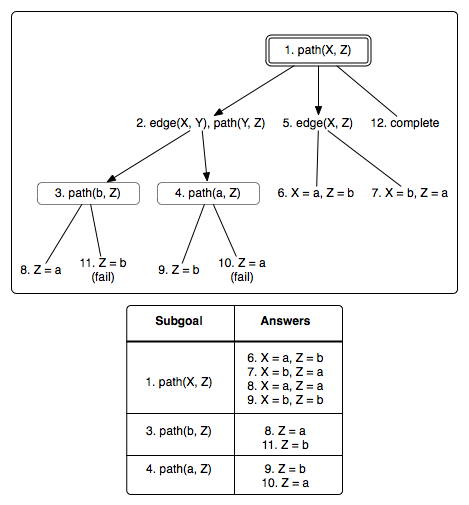
\includegraphics[scale=0.6]{tabling_path_sub.png}
  \caption{Tabling \textbf{path(X, Z)} using call by subsumption.}
  \label{fig:tabling_path_sub}
\end{figure}

At step 1 the subgoal \textbf{path(X, Z)} is called and a new generator node is created as there is no existing subgoals in the table space
that could be variant or subsuming. Being a generator node, it is evaluated using the program clauses (step 2). The first solution
for the \textbf{edge(X, Y)} predicate is evaluated using Prolog's standard rules and yields a subgoal call to \textbf{path(b, Z)} (step 3).

In variant tabling the engine would search for a variant subgoal in the table space, thus failing and creating a new generator node,
meanwhile expanding the execution tree by means of program clause resolution. In subsumptive tabling, the engine searches for a subsuming call,
and finds \textbf{path(X, Z)}. This subgoal
is more general than \textbf{path(b, Z)} and contains all the answers need for the subsumed goal.
A special type of consumer called a \textit{subsumptive consumer} is created. This consumer knows the subsuming subgoal and can retrieve
the answers that unify with the subsumed call.

As \textbf{path(X, Z)} has no answers and thus, no answers that can be consumed by \textbf{path(b, Z)}, the consumer node is suspended
and execution backtracks to node 2. The second clause of \textbf{edge/2} is tried and a new tabled subgoal is called: \textbf{path(a, Z)} (step 4).
Like \textbf{path(b, Z)}, this subgoal is subsumed by \textbf{path(X, Z)}, hence a new subsumptive consumer node is created. Execution suspends
once again because no answers are available and the engine goes back to node 1 to try the second \textbf{path/2} clause (step 5).

Solutions for \textbf{path(X, Z)} are found in steps 6 and 7, \textbf{X = a, Z = b} and \textbf{X = b, Z = a}, and stored in the answer set
for this generator node. Execution thus backtracks to node 1 and completion is attempted. Node 1 verifies that node 3 and 4 have
unconsumed answers and starts by resuming computation at node 3.

Node 3 being a subsumptive consumer looks up in the \textbf{path(X, Z)}
answer set for answers specific to \textbf{path(b, Z)}, finding one: \textbf{Z = a} (step 8). At this point, the consumer stores the answer
for later retrieval, so that answers can be immediately consumed when a variant subgoal is called.
Like variant tabling, the consumer keeps a last consumed answer continuation to know which answers have already been consumed.
Once the answer is stored, the variable bindings are propagated and a new answer to \textbf{path(X, Z)} is found: \textbf{X = a, Z = a}.
Node 3 tries to consume a new answer, but no new answers are available for this subgoal.

Execution suspends node 3 and resumes computation at node 4. Here \textbf{path(a, Z)} begins to consume answers from \textbf{path(X, Z)}
using the subsumption mechanism. The first answer in \textbf{path(X, Z)}, \textbf{X = a, Z = b}, unifies with the subsumed goal and
is consumed (step 9). By variable propagation, a new answer for \textbf{path(X, Z)} is also generated, \textbf{X = b, Z = b}.
Node 3 then tries to consume a new answer and finds \textbf{X = a, Z = a} (step 10). This new answer
is added to the \textbf{path(a, Z)} table space. As the new variable bindings are propagated, a new answer is also generated
for top subgoal, but the answer is repeated (\textbf{X = b, Z = a}), hence is not inserted into the table space.

As each consumer uses the available answers, execution backtracks to the leader node, \textbf{path(X, Z)}, that will once
again attempt completion. By using the last consumed answer continuation, it is verified that node 3 has unconsumed answers.
Execution thus resumes at node 3.

Node 3 inspects \textbf{path(X, Z)} answer set and consumes the next matching answer, \textbf{X = b, Z = b} (step 11). A new answer
for \textbf{path(b, Z)} is generated and variable bindings are propagated to the leader node. The new answer is already
stored in the table space and it is not used.

Once again, evaluation returns to the leader node and completion is attained (step 12) as each consumer has exhausted the
available answers.

This evaluation example, when compared to variant tabling, shows a smaller execution tree with less
program clauses expanded. The subsumptive computation also took less steps to complete and a greater
reuse of answers was done between \textbf{path(X, Z)}, \textbf{path(b, Z)} and \textbf{path(a, Z)}.

Although this example shows a very good performance of this method of evaluation, if we tried
to evaluate \textbf{path(a, Z)} and then \textbf{path(X, Z)}, no reuse could be done with \textbf{path(a, Z)}
because not previous subsuming goal was present. The more general subgoals are called first, the greater
the reuse in call subsumption.

Like variant tabling, the same four main operations are used when evaluating subsumptive subgoals.
These operations are very similar, with a few differences. Operations \textit{new answer} and
\textit{completion} remain the same, while the \textit{tabled subgoal call} and \textit{answer resolution}
work differently:

\begin{itemize}
  \item The \textit{tabled subgoal call} operation represents a call to a tabled subgoal.
  If the subgoal $c$ is called, a search for a subsuming subgoal $c'$ is done. If such subgoal is found,
  the new subgoal will be resolved using \textit{answer clause resolution}, thus consuming answers from the subgoal $c'$.
  If no subgoal $c'$ is found, then $c$ is inserted into the table space and the new generator node is evaluated using
  program clause resolution.
  
  \item The \textit{answer resolution} operation checks wether new answers from the table space are available for consumption.
  Each subsumptive consumer node uses an answer continuation that represents
  the set of remaining answers to be consumed. Given an answer continuation we inspect the answer trie from the subsuming subgoal
  and retrieve the next answer $T$ that matches with the subsumed goal. Once the answer is retrieved and loaded, the answer
  continuation is updated to reflect the new answer consumed.
\end{itemize}

The next sections describe two known techniques that implement subsumptive tabling. These two approaches were all implemented in XSB.

  \subsection{Dynamic Threaded Sequential Automata}
  \subsection{Time Stamped Tries} \label{sec:time_stamped_tries}
